\textcolor{black}{\section{Resultados y Análisis}}
Al graficar los datos de corriente y voltaje del diodo en polarización directa se obtiene la grafica que se muestra en figura (\ref{PD}), con su respectiva incertidumbre asociada a cada valor. Donde podemos observar que para voltajes $V_d$ inferiores a aproximadamente 0.4V la $I_d \approx 0 $ mientras que para ($V_d>0.4V$) la corriente empieza a crecer de manera exponencial. Mostrando el comportamiento característico de la unión de materiales tipo p-n.
\begin{figure}[htbp]
	\centering
	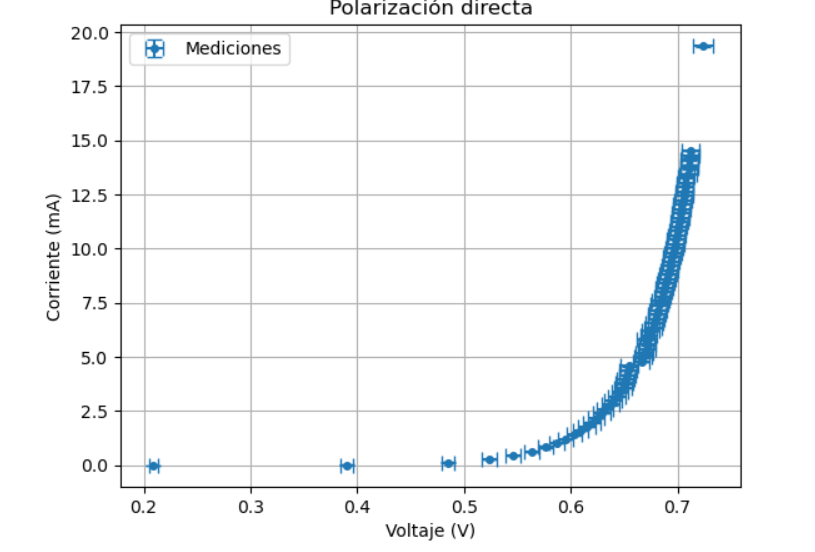
\includegraphics[scale=0.35]{figs/PD.png}
	\caption{Curva característica de corriente-voltaje ($I_d vs V_d$) del diodo en polarizacion directa}
	\label{PD}
\end{figure}
\FloatBarrier

Para obtener la relación $e/k_b$ a partir de la ecuación linealizada (\ref{shock3}) se graficó $ln(I_d)$ en función de $V_d$, obteniendo el ajuste lineal que se muestra en la figura (\ref*{log-log}): 
\begin{figure}[htbp]
	\centering
	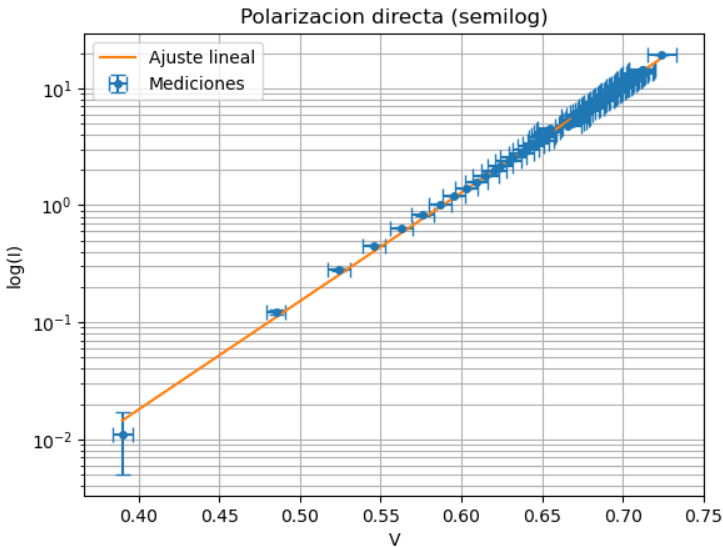
\includegraphics[scale=0.35]{figs/semilog.png}
	\caption{Linealización semilogarítmica de la ecuación de Shockley}
	\label{log-log}
\end{figure}
\FloatBarrier

De lo cual se obtiene una pendiente $m=42.7 \pm 1.48V^{-1}$. Utilizando la temperatura registrada de $T=299.15\pm 0.005 K$ y considerando que el diodo opera en la región de difusión ($n \approx1$). El resultado calculado así como el valor teórico esperado con su error relativo ($\epsilon_r$), así como también la incertidumbre de la pendiente ($\sigma$) se encuentran en la tabla (\ref{dat}):
\begin{table}[htbp] 
	\centering
    \begin{tabular}{|c|c|c|}
	    \hline
	    Magnitud & Valor & Unidad \\
	    \hline
		T &  299.15 $\pm 0.005$ & K\\
		\hline
		$e/k_b$  & 11604.518 & K/V \\
		(Teórico) &  & \\
		\hline
		$e/k_b$ & 12773.325  & K/V \\
		(Experimental) & $\pm 443$ & \\
		\hline
		$\epsilon_r$ & 10.1\%  & \\
		\hline
		$\sigma$ & 1.48 & \\
		\hline
		$R^2$ & 0.998 & \\
		\hline
 	\end{tabular}
 	\caption{ Parámetros experimentales, teóricos e incertidumbres derivados del ajuste lineal}
 	\label{dat}
\end{table}
\FloatBarrier

Los resultados obtenidos muestran una diferencia que se puede atribuir a diversas fuentes de error como el cambio de la temperatura ambiente a lo largo del trabajo, la resolución de los multímetros así como a la suposición de que la corriente del diodo es mucho mayor a la corriente de saturación ($I_d >> I_s$).

Posteriormente al colocar el diodo en polarización inversa los datos obtenidos se muestran en la figura (\ref{Pin}) 
\begin{figure}[htbp]
	\centering
	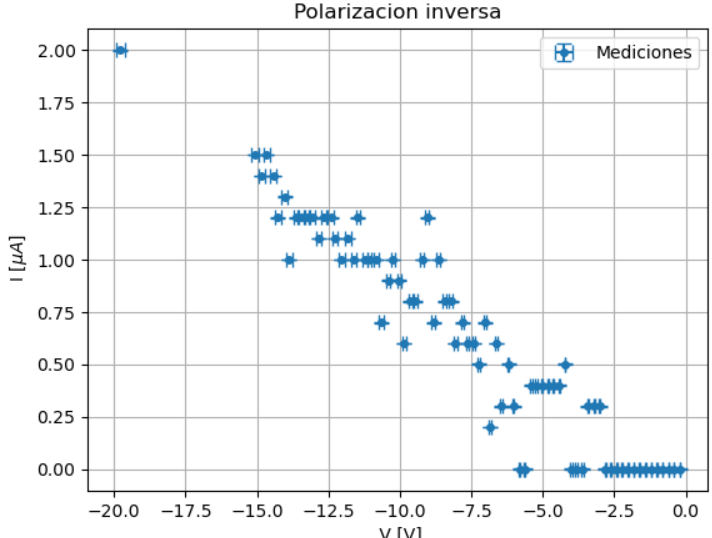
\includegraphics[scale=0.35]{figs/Pin.png}
	\caption{Mediciones de $I_d vs V_d$ del diodo en polarización inversa}
	\label{Pin}
\end{figure}
\FloatBarrier

En esta figura se observa que la polarización inversa no tiene un crecimiento exponencial de la corriente con el voltaje, mas bien se mantiene prácticamente constante en el orden de los microamperios, correspondiente a la corriente de saturación inversa. La dispersión en los puntos se debe a limitaciones de resolución en los instrumentos de medición, así como también al ruido presente en el montaje 
\noindent 